\begin{abox}
	Classical Mechanics
	\end{abox}
\begin{enumerate}
	\item Two particles of masses $m_{1}$ and $m_{2}$ are connected by a massless thread of length $l$ as shown in figure below.
	\begin{figure}[H]
		\centering
		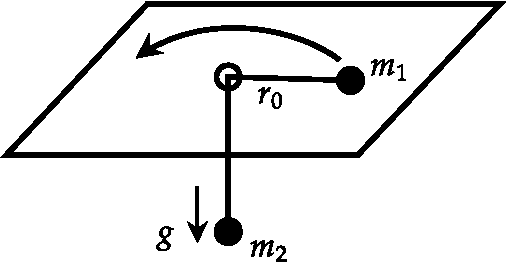
\includegraphics[height=2.8cm,width=5.3cm]{CM-01}
	\end{figure}
	The particle of mass in on the plane undergoes a circular motion with radius $r_{0}$ and angular momentum $L$. When a small radial displacement $\in\left(\right.$ whew $\in<<r_{0}$ ) is applied, its radial coordinate is found to found to oscillate about $r_{0}$. The frequency of the oscillations is
	NET/JRF (June-2019)
	 \begin{tasks}(2)
		\task[\textbf{a.}]$\sqrt{\frac{7 m_{2} g}{\left(m_{1}+\frac{m_{2}}{2}\right) r_{0}}}$
		\task[\textbf{b.}]$\sqrt{\frac{7 m_{2} g}{\left(m_{1}+m_{2}\right) r_{0}}}$
		\task[\textbf{c.}]$\sqrt{\frac{3 m_{2} g}{\left(m_{1}+\frac{m_{2}}{2}\right) r_{0}}}$
		\task[\textbf{d.}] $\sqrt{\frac{3 m_{2} g}{\left(m_{1}+m_{2}\right) r_{0}}}$
	\end{tasks}
\begin{answer}
	\begin{align*}
	L&=\frac{1}{2}\left(m_{1}+m_{2}\right) \ddot{r}+\frac{1}{2} m_{1} r^{2} \dot{\theta}^{2}-m_{2} g(l-r)\\
	\text{Lagrangian equation of motion; }&\frac{d}{d t}\left(\frac{\partial L}{\partial \dot{r}}\right)-\frac{\partial L}{\partial r}=0\\
	\left(m_{1}+m_{2}\right) \ddot{r}-m_{1} r \dot{\theta}^{2}+m_{2} g&=0
	\intertext{Hence angular momentum is conserved}
	m_{1} r^{2} \dot{\theta}&=m_{1} r_{0}^{2} \dot{\theta}_{0} \Rightarrow \dot{\theta}=\frac{r_{0}^{2} \dot{\theta}_{0}}{r^{2}}\\
	\text{For circular motion }&m r_{0} \dot{\theta}_{0}^{2}=m_{2} g\\
	\text{	so }r \dot{\theta}^{2}&=\frac{m_{2}}{m_{1}}\left(\frac{r_{0}}{r}\right)^{3} g\\
	\left(m_{1}+m_{2}\right) \ddot{r}-m_{2}\left(\frac{r_{0}}{r}\right)^{3} g+m_{2} g&=0\\
	\text{Put }r&=r_{0}+\in \ddot{r}=\ddot{\epsilon}\\
	\intertext{$\left(m_{1}+m_{2}\right) \ddot{\in}-m_{2}\left(\frac{r_{0}}{r_{0}+\epsilon}\right)^{3} g+m_{2} g\Rightarrow\left(m_{1}+m_{2}\right) \ddot{\in}-m_{2} r_{0}^{3}\left(r_{0}+\epsilon\right)^{-3} g+m_{2} g$}\\
	\left(m_{1}+m_{2}\right) \ddot{\star}-m_{2} r_{0}^{3} g r_{0}^{-3}\left(1+\frac{\epsilon}{r_{0}}\right)^{-3}+m_{2} g&=0\\
	\left(m_{1}+m_{2}\right) \ddot+\frac{m_{2} 3 \epsilon}{r_{0}}&=0 \Rightarrow \omega=\sqrt{\frac{3 m_{2} g}{\left(m_{1}+m_{2}\right) r_{0}}}
	\end{align*}
	So the correct answer is \textbf{Option (D)}
\end{answer}
	\item The spring constant $k$ of a spring of mass $m_{s}$ is determined experimentally by loading the spring with mass $M$ and recording the time period $T$, for a single oscillation. If the experiment is carried out for different masses, then the graph that correctly represents the result is
{	\exyear{NET/JRF(DEC-2017)}}
\begin{tasks}(2)
\task[\textbf{A.}] \begin{figure}[H]
	\centering
	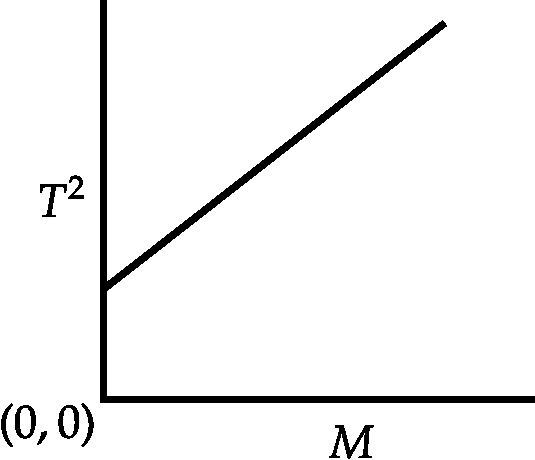
\includegraphics[height=3cm,width=4.5cm]{CM-2}
\end{figure}
\task[\textbf{B.}] \begin{figure}[H]
	\centering
	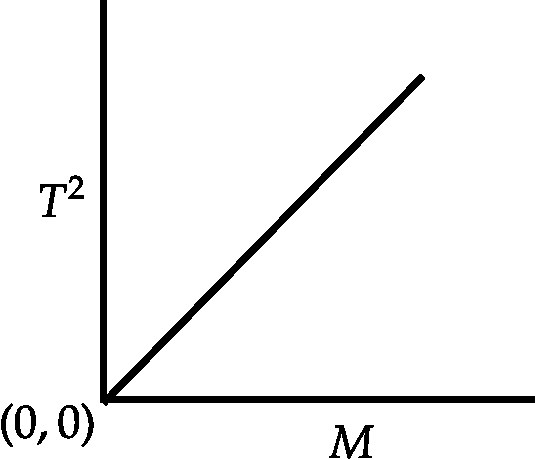
\includegraphics[height=3cm,width=4.5cm]{CM-3}
\end{figure}
\task[\textbf{C.}] \begin{figure}[H]
	\centering
	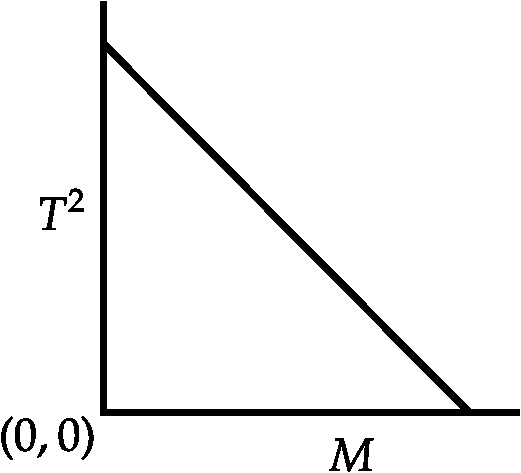
\includegraphics[height=3cm,width=4.5cm]{CM-4}
\end{figure}
\task[\textbf{D.}] \begin{figure}[H]
	\centering
	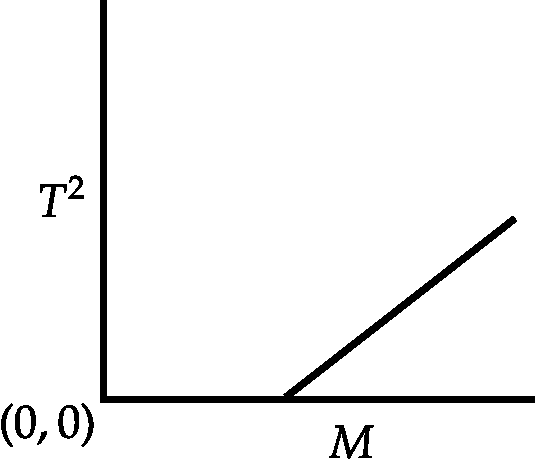
\includegraphics[height=3cm,width=4.5cm]{CM-5}
\end{figure}
\end{tasks}
\begin{answer}
\begin{align*}
\intertext{The Langragian of system.}
L&=\frac{1}{2} \cdot \frac{m_{s}}{3} \dot{x}^{2}+\frac{1}{2} M \dot{x}^{2}-\frac{1}{2} k x^{2}, \frac{d}{d t}\left(\frac{\partial L}{\partial \dot{x}}\right)-\frac{\partial L}{\partial x}=0\\
\frac{d}{d t} \frac{\partial L}{\partial x}&=0 \Rightarrow\left(\frac{m_{s}}{3}+M\right) \ddot{x}=-k x\\
T&=2 \pi \sqrt{\frac{M+\frac{m_{s}}{3}}{k}} \Rightarrow T^{2}=4 \pi \frac{\left(M+\frac{m_{s}}{3}\right)}{k}
\end{align*}
So the correct answer is \textbf{Option (A)}
\end{answer}
	\item Two coupled oscillators in a potential $V(x, y)=\frac{1}{2} k x^{2}+2 x y+\frac{1}{2} k y^{2}(k>2)$ can be decoupled into two independent harmonic oscillators (coordinates: $x^{\prime}, y^{\prime}$ ) by means of an appropriate transformation $\left(\begin{array}{c}x^{\prime} \\ y^{\prime}\end{array}\right)=S\left(\begin{array}{l}x \\ y\end{array}\right) .$ The transformation matrix $S$ is
	{\exyear{NET/JRF(JUNE-2020)}}
\begin{tasks}(2)
\task[\textbf{A.}] $\left(\begin{array}{cc}\frac{1}{\sqrt{2}} & 1 \\ 1 & -\frac{1}{\sqrt{2}}\end{array}\right)$
\task[\textbf{B.}] $\left(\begin{array}{ll}\frac{1}{\sqrt{2}} & -\frac{1}{\sqrt{2}} \\ \frac{1}{\sqrt{2}} & \frac{1}{\sqrt{2}}\end{array}\right)$
\task[\textbf{C.}] $\left(\begin{array}{cc}\frac{1}{\sqrt{2}} & -\frac{1}{\sqrt{2}} \\ -\frac{1}{\sqrt{2}} & \frac{1}{\sqrt{2}}\end{array}\right)$
\task[\textbf{D.}] $\left(\begin{array}{cc}0 & -1 \\ 1 & 0\end{array}\right)$
\end{tasks}
\begin{answer}
\begin{align*}
\intertext{ The normal mode of given potential is $\left(\begin{array}{l}\frac{1}{\sqrt{2}} \\ \frac{1}{\sqrt{2}}\end{array}\right)$ and $\left(\begin{array}{l}-\frac{1}{\sqrt{2}} \\ \frac{1}{\sqrt{2}}\end{array}\right)$ in the basis of normal mode the potential can be diagonalise.}
\end{align*}
So the correct answer is \textbf{Option (B)}
\end{answer}
	\item  A particle moves in the one-dimensional potential $V(x)=\alpha x^{6}$, where $a>0$ is a constant. If the total energy of the particle is $E$, its time period in a periodic motion is proportional to
{	\exyear{NET/JRF(JUNE-2018)}}
\begin{tasks}(4)
\task[\textbf{A.}] $E^{-1 / 3}$
\task[\textbf{B.}] $E^{-1 / 2}$
\task[\textbf{C.}] $E^{1 / 3}$
\task[\textbf{D.}] $E^{1 / 2}$
\end{tasks}
\begin{answer}
\begin{align*}
J&=\oint P d x\\
&J \propto(2 m E)^{1 / 2}\left(\frac{E}{a}\right)^{1 / 6} \quad \Rightarrow E \propto J^{3 / 2} \\ v&=\frac{d E}{d J} \propto J^{1 / 2} \Rightarrow v \propto E^{1 / 3} \quad \Rightarrow T \propto E^{-1 / 3}
\end{align*}
So the correct answer is \textbf{Option (A)}
\end{answer}
	\item A particle of mass $m$, kept in potential $V(x)=-\frac{1}{2} k x^{2}+\frac{1}{4} \lambda x^{4}$ (where $k$ and $\lambda$ are positive constants), undergoes small oscillations about an equilibrium point. The frequency of oscillations is
	{\exyear{NET/JRF(JUNE-2018)}}
\begin{tasks}(2)
\task[\textbf{A.}] $\frac{1}{2 \pi} \sqrt{\frac{2 \lambda}{m}}$
\task[\textbf{B.}] $\frac{1}{2 \pi} \sqrt{\frac{k}{m}}$
\task[\textbf{C.}] $\frac{1}{2 \pi} \sqrt{\frac{2 k}{m}}$
\task[\textbf{D.}] $\frac{1}{2 \pi} \sqrt{\frac{\lambda}{m}}$
\end{tasks}
\begin{answer}
\begin{align*}
V&=-\frac{1}{2} k x^{2}+\frac{1}{4} \lambda x^{4}\\
\frac{d V}{d x}&=0 \quad-k x+\lambda x^{3}=0\\
x&=0, \quad x^{2}=\frac{k}{\lambda} \Rightarrow x=x_{0}=\sqrt{\frac{k}{\lambda}}\\
\frac{d^{2} V}{d x^{2}}&=-k \quad\text{ at $x=0 \quad$ so $x=0$ is unstable part}\\
\frac{d^{2} V}{d x^{2}}&=2 k\text{ at $x_{0}=\sqrt{\frac{k}{\lambda}}$ so $x_{0}=\sqrt{\frac{k}{x}}$ is stable equation point}\\
\omega&=\sqrt{\frac{\left.\frac{d^{2} V}{d x^{2}}\right|_{x=x_{0}}}{m}}=\sqrt{\frac{2 k}{m}} \quad f=\frac{1}{2 \pi} \sqrt{\frac{2 k}{m}}
\end{align*}
So the correct answer is \textbf{Option (C)}
\end{answer}
	\item A rod pivoted at one end is rotating clockwise 25 times a second in a plane. A video camera which records at a rate of 30 frames per second is used to film the motion. To someone watching the video, the apparent motion of the rod will seem to be
{	\exyear{NET/JRF(JUNE-2020)}}
\begin{tasks}(1)
\task[\textbf{A.}] 10 rotations per second in the clockwise direction
\task[\textbf{B.}]  10 rotations per second in the anticlockwise direction
\task[\textbf{C.}] 5 rotations per second in the clockwise direction
\task[\textbf{D.}] 5 rotations per second in the anticlockwise direction
\end{tasks}
\begin{answer}
So the correct answer is \textbf{Option (D)}
\end{answer}
	\item An annulus of mass $M$ made of a material of uniform density has inner and outer radii $a$ and $b$ respectively. Its principle moment of inertia along the axis of symmetry perpendicular to the plane of the annulus is:
{	\exyear{NET/JRF(DEC-2011)}}
\begin{tasks}(4)
\task[\textbf{A.}] $\frac{1}{2} M \frac{\left(b^{4}+a^{4}\right)}{\left(b^{2}-a^{2}\right)}$
\task[\textbf{B.}] $\frac{1}{2} M \pi\left(b^{2}-a^{2}\right)$
\task[\textbf{C.}]  $\frac{1}{2} M\left(b^{2}-a^{2}\right)$
\task[\textbf{D.}] $\frac{1}{2} M\left(b^{2}+a^{2}\right)$
\end{tasks}
\begin{answer}
So the correct answer is \textbf{Option (D)}
\end{answer}
	\item Two bodies of equal mass $m$ are connected by a massless rigid rod of length $l$ lying in the $x y$-plane with the centre of the rod at the origin. If this system is rotating about the $z$-axis with a frequency $\omega$, its angular momentum is
{	\exyear{NET/JRF(DEC-2012)}}
\begin{tasks}(4)
\task[\textbf{A.}] $m l^{2} \omega / 4$
\task[\textbf{B.}] $m l^{2} \omega / 2$
\task[\textbf{C.}] $m l^{2} \omega$
\task[\textbf{D.}]  $2 m l^{2} \omega$
\end{tasks}
\begin{answer}
\begin{align*}
\intertext{Since rod is massless i.e. $M=0$.}
\text{Moment of inertia of the system }I&=m_{1} r_{1}^{2}+m_{2} r_{2}^{2}, m_{1}\\&=m_{2}=m\text{ and }r_{1}=r_{2}=\frac{l}{2}\\
I&=\frac{m l^{2}}{4}+\frac{m l^{2}}{4} \Rightarrow I=\frac{m l^{2}}{2}.\\\text{ Angular momentum, }J&=I \omega\text{ and }J=\frac{m l^{2} \omega}{2}.
\end{align*}
So the correct answer is \textbf{Option (B)}
\end{answer}
	\item A particle of mass $m$ moves in a central potential $V(r)=-\frac{k}{r}$ in an elliptic orbit $r(\theta)=\frac{a\left(1-e^{2}\right)}{1+e \cos \theta}$, where $0 \leq \theta<2 \pi$ and $a$ and $e$ denote the semi-major axis and eccentricity, respectively. If its total energy is $E=-\frac{k}{2 a}$, the maximum kinetic energy is
{	\exyear{NET/JRF(JUNE-2018)}}
\begin{tasks}(4)
\task[\textbf{A.}] $E\left(1-e^{2}\right)$
\task[\textbf{B.}] $E \frac{(e+1)}{(e-1)}$
\task[\textbf{C.}] $E /\left(1-e^{2}\right)$
\task[\textbf{D.}] $E \frac{(e-1)}{(e+1)}$
\end{tasks}
\begin{answer}
\begin{align*}
E&=T+V \quad T=E-V\\
T&=-\frac{k}{2 a}+\frac{k}{r} T\\&=-\frac{k}{2 a}+\frac{k}{a\left(1-e^{2}\right)}(1+\cos \theta)\\
T.\text{ maximum }\cos \theta&=1\\
T_{\max }&=-\frac{k}{2 a}+\frac{k(1+e)}{a\left(1-e^{2}\right)}\\&=-\frac{k}{2 a}+\frac{k}{a} \frac{(1+e)}{(1-e)(1+e)}\\
&=-\frac{k}{a}\left[\frac{1}{2}+\frac{1}{(1-e)}\right]\\&=-\frac{k}{2 a}\left(\frac{1+e}{1-e}\right)=E\left(\frac{1+e}{1-e}\right)
\end{align*}
So the correct answer is \textbf{Option (B)}
\end{answer}
	\item Consider circular orbits in a central force potential $V(r)=-\frac{k}{r^{n}}$, where $k>0$ and $0<n<2$. If the time period of a circular orbit of radius $R$ is $T_{1}$ and that of radius $2 R$ is $T_{2}$, then $\frac{T_{2}}{T_{1}}$
{	\exyear{NET/JRF(DEC-2016)}}
\begin{tasks}(4)
\task[\textbf{A.}] $2^{\frac{n}{2}}$
\task[\textbf{B.}] $2^{\frac{2}{3} n}$
\task[\textbf{C.}] $2^{\frac{n}{2}+1}$
\task[\textbf{D.}]  $2^{n}$
\end{tasks}
\begin{answer}
\begin{align*}
V_{e f f}&=\frac{J^{2}}{2 m r^{2}}-\frac{k}{r^{n}}, \frac{\partial V_{e f f}}{\partial r}=-\frac{J^{2}}{m r^{3}}+\frac{n k}{r^{n+1}}=0\\
\because J&=m r^{2} \omega \quad \Rightarrow \frac{m^{2} \omega^{2} r^{4}}{r^{3}}=\frac{n k}{r^{n+1}} \\&\Rightarrow \omega^{2} \propto \frac{1}{r^{n+2}} \Rightarrow \omega \propto r^{-(n+2) / 2} \Rightarrow T \propto r^{\frac{n}{2}+1}\\
\frac{T_{2}}{T_{1}}=\left(\frac{2 R}{R}\right)^{\frac{n+2}{2}}=2^{\frac{n}{2}+1}
\end{align*}
So the correct answer is \textbf{Option (C)}
\end{answer}
	\item A planet of mass $m$ and an angular momentum $L$ moves in a circular orbit in a potential, $V(r)=-k / r$, where $k$ is a constant. If it is slightly perturbed radially, the angular frequency of radial oscillations is
{	\exyear{NET/JRF(JUNE-2013)}}
\begin{tasks}(4)
\task[\textbf{A.}] $m k^{2} / \sqrt{2} L^{3}$
\task[\textbf{B.}] $m k^{2} / L^{3}$
\task[\textbf{C.}] $\sqrt{2} m k^{2} / L^{3}$
\task[\textbf{D.}] $\sqrt{3} m k^{2} / L^{3}$
\end{tasks}
\begin{answer}$\left. \right. $
\begin{figure}[H]
	\centering
	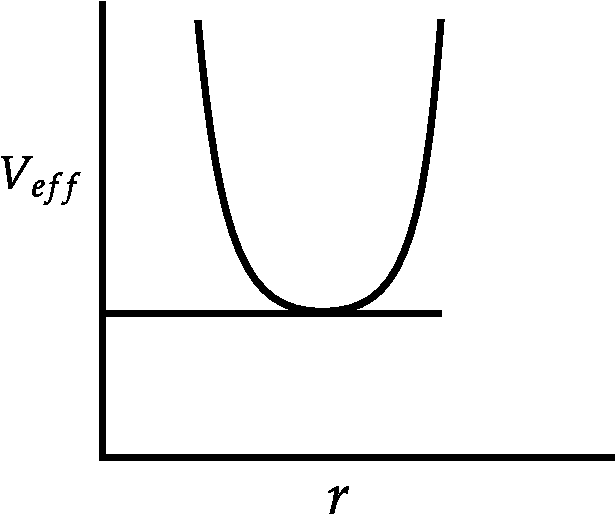
\includegraphics[height=4cm,width=5cm]{CM-6}
\end{figure}
\begin{align*}
V_{e f f}&=\frac{L^{2}}{2 m r^{2}}-\frac{k}{r} .\text{ For circular orbit }\frac{\partial V_{e f f}}{\partial r}=-\frac{L^{2}}{m r^{3}}+\frac{k}{r^{2}}=0\\
\Rightarrow \frac{L^{2}}{m r^{3}}&=\frac{k}{r^{2}} .\text{ Thus }r=r_{0}=\frac{L^{2}}{m k} \Rightarrow \omega=\sqrt{\frac{k}{m}}\\
k&=\left.\frac{d^{2} V_{e f f}}{d r^{2}}\right|_{r=r_{0}}=+\frac{3 L^{2}}{m r^{4}}-\left.\frac{2 k}{r^{3}}\right|_{r=r_{0}}\\&=\frac{3 L^{2}}{m\left(\frac{L^{2}}{m k}\right)^{4}}-\frac{2 k}{\left(\frac{L^{2}}{m k}\right)^{3}}=\frac{3 m^{3} k^{4}}{L^{6}}-\frac{2 m^{3} k^{4}}{L^{6}}=\frac{m^{3} k^{4}}{L^{6}}\\
\omega&=\sqrt{\frac{\left.\frac{d^{2} V}{d r^{2}}\right|_{r=r_{0}}}{m}} \Rightarrow \omega=\frac{m k^{2}}{L^{3}}
\end{align*}
So the correct answer is \textbf{Option (B)}
\end{answer}
	\item Consider a set of particles which interact by a pair potential $V=a r^{6}$ where $r$ is the interparticle separation and $a>0$ is a constant. If a system of such particles has reached virial equilibrium, the ratio of the kinetic to the total energy of the system is
{	\exyear{NET/JRF(DEC-2017)}}
\begin{tasks}(4)
\task[\textbf{A.}] $\frac{1}{2}$
\task[\textbf{B.}] $\frac{1}{3}$
\task[\textbf{C.}] $\frac{3}{4}$
\task[\textbf{D.}] $\frac{2}{3}$
\end{tasks}
\begin{answer}
\begin{align*}
V(r)&=a r^{n}\langle T\rangle=\frac{n}{2}\langle V\rangle\\
V\langle r\rangle&=a r^{6}\text{ and }\langle T\rangle=3\langle V\rangle\\
\text{Then, }\langle E\rangle&=\langle T\rangle+\langle V\rangle=\langle T\rangle+\frac{1}{3}\langle T\rangle \Rightarrow\langle E\rangle\\&=\frac{4}{3}\langle T\rangle \Rightarrow \frac{\langle T\rangle}{\langle E\rangle}=\frac{3}{4}
\end{align*}
So the correct answer is \textbf{Option (C)}
\end{answer}
	\item Which of the following figures best describes the trajectory of a particle moving in a repulsive central potential $V(r)=\frac{a}{r}(a>0$ is a constant)?
{	\exyear{NET/JRF(JUNE-2018)}}
\begin{tasks}(2)
\task[\textbf{A.}] \begin{figure}[H]
	\centering
	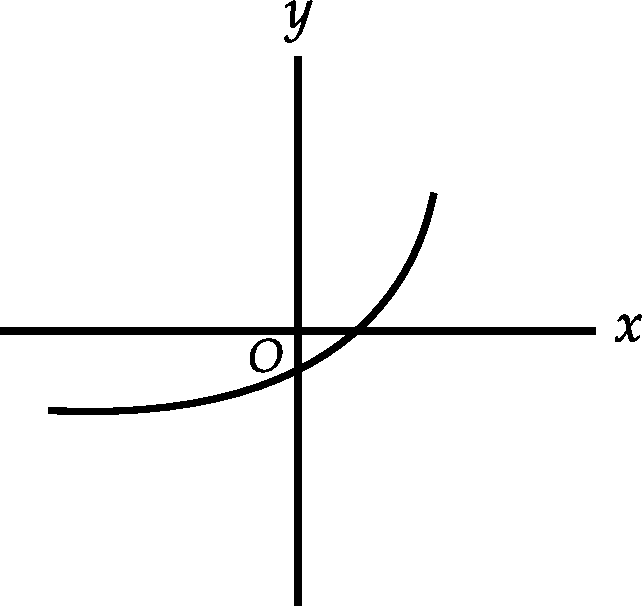
\includegraphics[height=4.5cm,width=5cm]{CM-7}
\end{figure}
\task[\textbf{B.}] \begin{figure}[H]
	\centering
	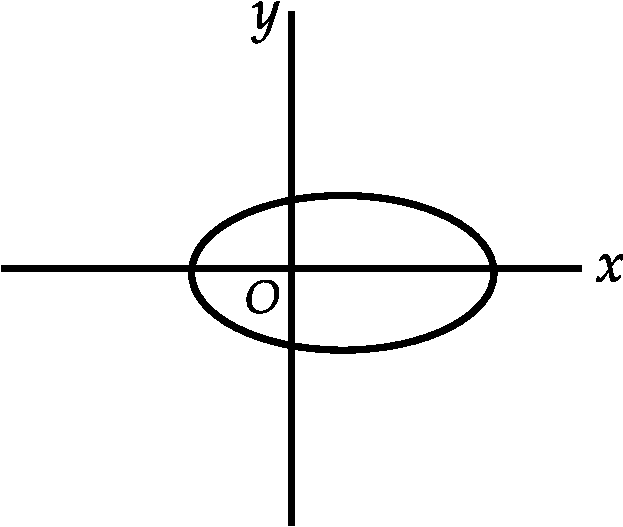
\includegraphics[height=4.5cm,width=5cm]{CM-8}
\end{figure}
\task[\textbf{C.}] \begin{figure}[H]
	\centering
	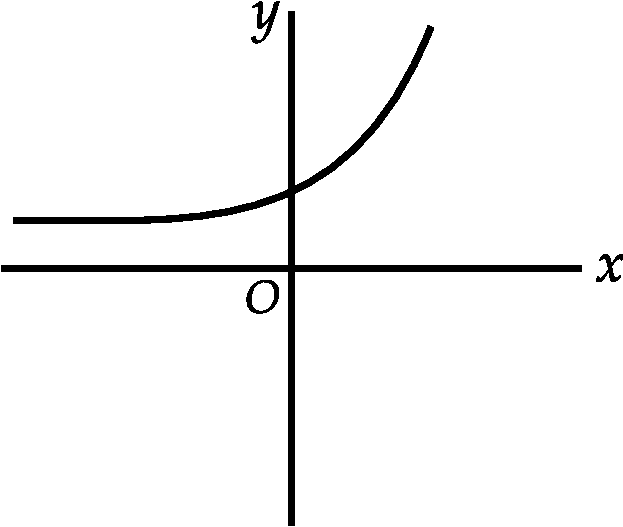
\includegraphics[height=4.5cm,width=5cm]{CM-9}
\end{figure}
\task[\textbf{D.}] \begin{figure}[H]
	\centering
	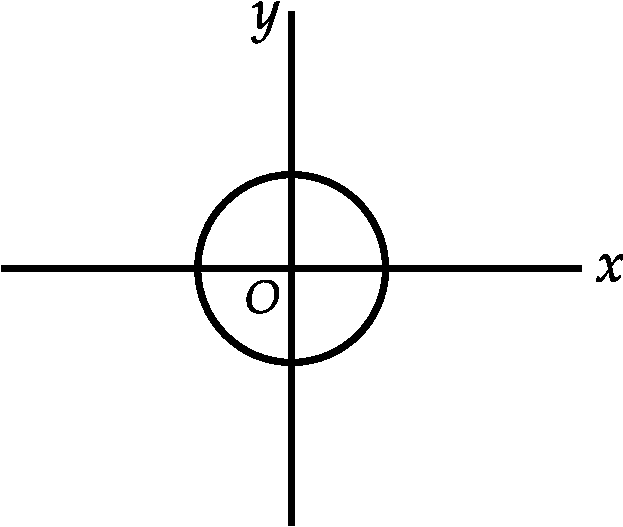
\includegraphics[height=4.5cm,width=5cm]{CM-10}
\end{figure}
\end{tasks}
\begin{answer}$\left. \right. $
\begin{figure}[H]
	\centering
	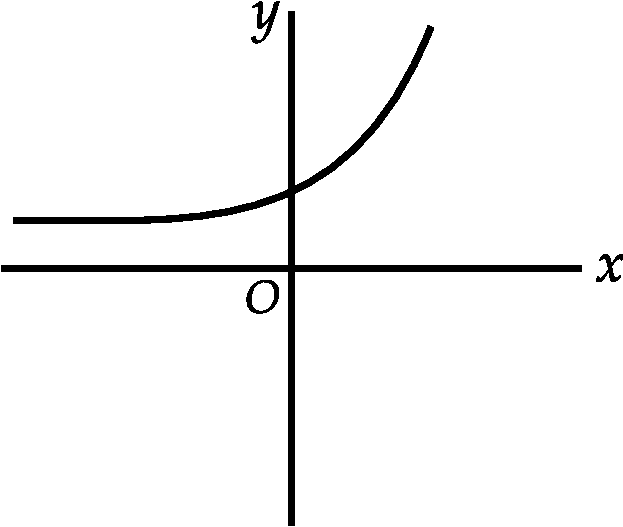
\includegraphics[height=4.5cm,width=5cm]{CM-11}
\end{figure}
\begin{align*}
\intertext{The potential is $V(r)=\frac{a}{r}$ which is repulsive. So there is unbounded motion and mainly represent by scattering project}
\end{align*}
So the correct answer is \textbf{Option (C)}
\end{answer}
	\item A horizontal circular platform mutes with a constant angular velocity $\Omega$ directed vertically upwards. A person seated at the centre shoots a bullet of mass $m$ horizontally with speed $v$. The acceleration of the bullet, in the reference frame of the shooter, is
{	\exyear{NET/JRF(JUNE-2012)}}
\begin{tasks}(2)
\task[\textbf{A.}]  $2 v \Omega$ to his right
\task[\textbf{B.}] $2 v \Omega$ to his left
\task[\textbf{C.}] $v \Omega$ to his right
\task[\textbf{D.}] $v \Omega$ to his left
\end{tasks}
\begin{answer}
\begin{align*}
\intertext{Velocity of bullet $=\hat{v j}$, Angular velocity $=\Omega \hat{k}$. There will be coriolis force $\vec{F}=2 m(\vec{v} \times \vec{\Omega})$}
\vec{F}&=2 m \Omega v \hat{i} \Rightarrow \vec{a}=2 v \Omega \hat{i}
\end{align*}
So the correct answer is \textbf{Option (A)}
\end{answer}
	\item A disc of mass $m$ is free to rotate in a plane parallel to the $x y$ plane with an angular velocity $-\omega \hat{z}$ about a massless rigid rod suspended from the roof of a stationary car (as shown in the figure below). The rod is free to orient itself along any direction. The car accelerates in the positive $x$-direction with an acceleration $a>0 .$ Which of the following statements is true for the coordinates of the centre of mass of the disc in the reference frame of the car?
{	\exyear{NET/JRF(DEC-2017)}}
\begin{figure}[H]
\centering
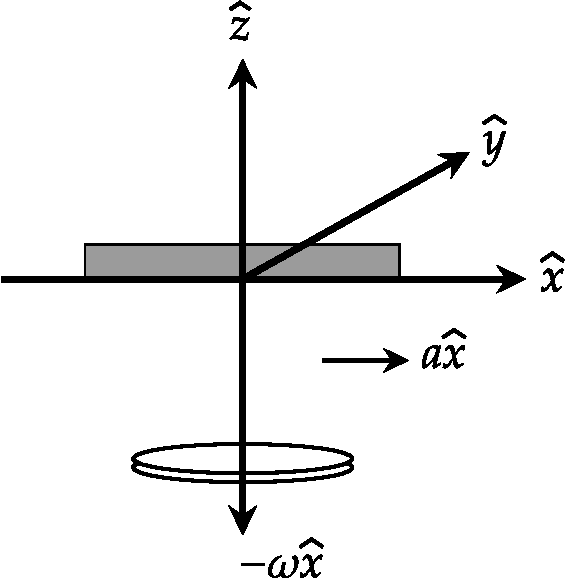
\includegraphics[height=5cm,width=5cm]{CM-12}
\end{figure}
\begin{tasks}(1)
\task[\textbf{A.}] Only the $x$ and the $z$ coordinates change
\task[\textbf{B.}] Only the $y$ and the $z$ coordinates change
\task[\textbf{C.}] Only the $x$ and the $y$ coordinates change
\task[\textbf{D.}] All the three coordinates change
\end{tasks}
\begin{answer}
So the correct answer is \textbf{Option (D)}
\end{answer}
	
	
	
\end{enumerate}